\documentclass[preprint]{aastex}
\usepackage{graphicx}
\usepackage{natbib}
\usepackage{wrapfig}
\usepackage{amsmath}
\usepackage{simplemargins}
%\setallmargins{0.8in}
\setleftmargin{0.75in}
\setrightmargin{0.75in}
\settopmargin{0.72in}
\setbottommargin{0.72in}
\bibliographystyle{apj}
\pagestyle{plain}

\renewcommand{\abstractname}{Summary}
\newcommand\etal{{\it et al.}}
\newcommand\eg{{\it e.g.,~}}
\newcommand\ie{{\it i.e.,~}}

\begin{document}

\title{\LARGE \bf Numerical Simulations of Dead Zone Turbulence}
\author{\large Jacob B. Simon (PI), Rebecca G. Martin, Philip J. Armitage, Daniel Gold}
\affil{JILA/University of Colorado, Boulder}
\maketitle
\vspace{-8mm}
\section{Summary}
We request a total of $\mathbf{2.85\times10^6}$ {\bf SUs} on the {\sc Janus} supercomputer to conduct numerical simulations of astrophysical accretion disks around young stars.
Utilizing the well-tested, publicly available, magnetohydrodynamics code {\sc Athena}, we will evolve local, co-rotating regions of these disks to explore how the level of turbulence near the disk mid-plane depends on the surface density of the disk.  Funding for the proposed research will be provided by the National Science Foundation through grant AST-1313021, by NASA through grant NNX13AI58G, and by two NASA Sagan Fellowships (PI Simon and co-I Martin). 

\vspace{-8mm}
\section{Introduction and Scientific Motivation}
\vspace{-2mm}
Disks around young stars play a crucial role in star and planet formation processes.  These {\it protoplanetary disks} actively accrete their gas onto the central star, contributing to the young star's growth, and contain the rocky building blocks for planets to form.  
Both the accretion of gas onto the star and the processes that produce planets are intimately tied to {disk turbulence} driven by the magnetorotational instability \cite[MRI;][]{balbus91,balbus98}.  

In fully ionized disks, such as those around black holes, the MRI is very efficient at producing turbulence and driving accretion.  However, protoplanetary disks are significantly colder than their black hole counterparts and consequently have a lower ionization fraction throughout large regions of the disk.  Since strong coupling of the gas to magnetic fields is crucial for the MRI to operate, there can be extensive regions of no MRI activity in such disks.  In fact, for radial distances larger than $\sim$0.1 AU\footnote{AU, or astronomical unit, is the distance between the Earth and the Sun.}, the temperature of the gas is simply too low for thermal ionization \citep{umebayashi83}.  Instead, the disk surface layers (far from the disk mid-plane) are ionized by cosmic rays \citep{gammie96}, stellar X-rays \citep{igea99}, and stellar FUV photons \citep{perez-becker11b}.

These non-thermal sources ionize the gas sufficiently well for the MRI to generate turbulence in the surface layers.  The result is a layered disk model for accretion; two ``active" layers surround a ``dead zone" region near the disk mid-plane \citep{gammie96}.  While in this basic model, the primary source of accretion occurs through the disk surface layers, numerical simulations \citep{fleming03,simon11b} have shown that these active surface layers can pump energy into the dead zone region, producing small but non-negligible levels of turbulence there.   

Recent work by co-I Martin has focused on the global evolution of protoplanetary disks using semi-analytic, 1D models that take into account the presence of the dead zone.  In these models, the dead zone extends radially from roughly 0.1 AU to 10 AU; at larger radii the disk surface density is low enough for the 
non-thermal ionization sources to ionize the entire vertical extent of the disk.  Thus, the dead zone acts like a plug in the accretion flow and gas builds up in this region.  This build up eventually causes the gas to become turbulent from gravitational instability, heating the gas and increasing its ionization fraction.  The increased ionization can then trigger the MRI, causing a much higher level of disk turbulence and accretion: an outburst. After an outburst, the remaining disk gas cools and is replenished by
accreting gas from larger radii \cite[e.g.,][]{armitage01,martin11,martin13,martin14}. The outburst then repeats at later times in an approximately periodic manner. This process is a potential mechanism for FU Ori outbursts in young stars.

On the numerical front, many studies have characterized the nature of the dead zone.  Recent work by PI Simon \citep{simon11b} shows that not only is there turbulence in the dead zone, but the level of this turbulence increases with height above the mid-plane.  Such simulations can inform 1D models of global disk evolution, such as those described above, by providing a framework with which to include dead zone turbulence. 

The primary limitation with numerical simulations of dead zones performed to-date is that they all use the same model for the disk surface density: the minimum mass solar nebula (MMSN).  The MMSN is a model for disks based on the distribution of mass (now locked up in planets, dwarf planets, and moons) in our own solar system.  However, both observations \cite[e.g.,][]{qi11} and 1D models \cite[e.g.,][]{martin12} suggest that the surface density can be larger than the MMSN by up to several orders of magnitude.  Yet the various sources of ionization always penetrate to a surface density of $\sim$10-100 g/cm$^2$ vertically.   A more massive disk implies a spatially larger dead zone relative to the active MRI region. This variation of dead zone to active region thickness could strongly affect the level of turbulence in the dead zone since the turbulent energy pumped from the active layers will be spread over a larger region.

The 1D models studied by co-I Martin assume that there is no turbulence in the dead zone layer. However, by including turbulence in the dead zone, the results of the 1D calculations will likely change significantly.  For example, if there is sufficient turbulence pumped into the dead zone from the active layers, the additional heating from this turbulence, instead of self-gravitating turbulence, may be responsible for triggering the MRI and the resulting outburst \citep{martin14}.  Thus, a proper understanding of how the level of turbulence in the dead zone scales with the disk surface density is crucial for vastly improving the accuracy of these models. The primary goal of the simulations proposed here is to uncover this relationship between surface density and dead zone turbulence through carefully crafted numerical simulations.

\vspace{-8mm}
\section{Proposed Computational Methods}
\label{sec:code}
\vspace{-2mm}

Our simulations will use the publicly available and extensively tested multidimensional MHD code {\sc Athena}\footnotemark.
\footnotetext{The {\sc Athena} code and a repository of test problems are maintained online at https://trac.princeton.edu/Athena/.}
The fundamental structure of {\sc Athena} is described in \citet{gardiner05a} and \citet{gardiner08} with detailed descriptions of the algorithms appearing in \citet{stone08} and \cite{stone10}.
For this project, we will be using {\sc Athena}, as presented in \citet{stone10}, to solve the equations of compressible MHD in the shearing box limit {\it including} Ohmic diffusion, which is responsible for the dead zone. 
This is accomplished with a dimensionally unsplit, second-order accurate integrator combined with a constrained transport method for evolving the magnetic induction equation and preserving a divergence-free magnetic field. 
Additionally, as elaborated upon in \citet{stone10}, certain modifications have been made to the code in the shearing box approximation in order to conserve vertical magnetic flux to machine precision, as well as to accurately capture the physics of epicyclic motion.  An orbital advection scheme has also been implemented to remove numerical diffusion created by the Keplerian shear flow and to increase the Courant limited time step.

{\sc Athena} is parallelized via domain decomposition through MPI.  The code has been optimized so that the number of MPI communication calls is on the order of once per time step; this leads to excellent scaling on large numbers of cores.  In particular, {\sc Athena} has been carefully benchmarked on a variety of large-scale computing systems, including a Cray XT-3 at Sandia National Lab ({\sc Red Storm}), a Cray XT-5 at NICS ({\sc Kraken}), a Sun Magnum at TACC ({\sc Ranger}), and {\sc Janus}. In all cases, it has shown nearly perfect scaling out to large numbers of cores. Figure 1 illustrates the code's weak scaling performance on {\sc Janus} and {\sc Ranger}, showing that the code runs at better than $93\%$ efficiency for $64^3$ zones/core, even out to $\sim 3000$ cores. Given its accuracy and efficiency, {\sc Athena} is an appropriate code for our interests.

\begin{wrapfigure}{r}{0.55\textwidth}
\vspace{-0.3cm}
\begin{center}
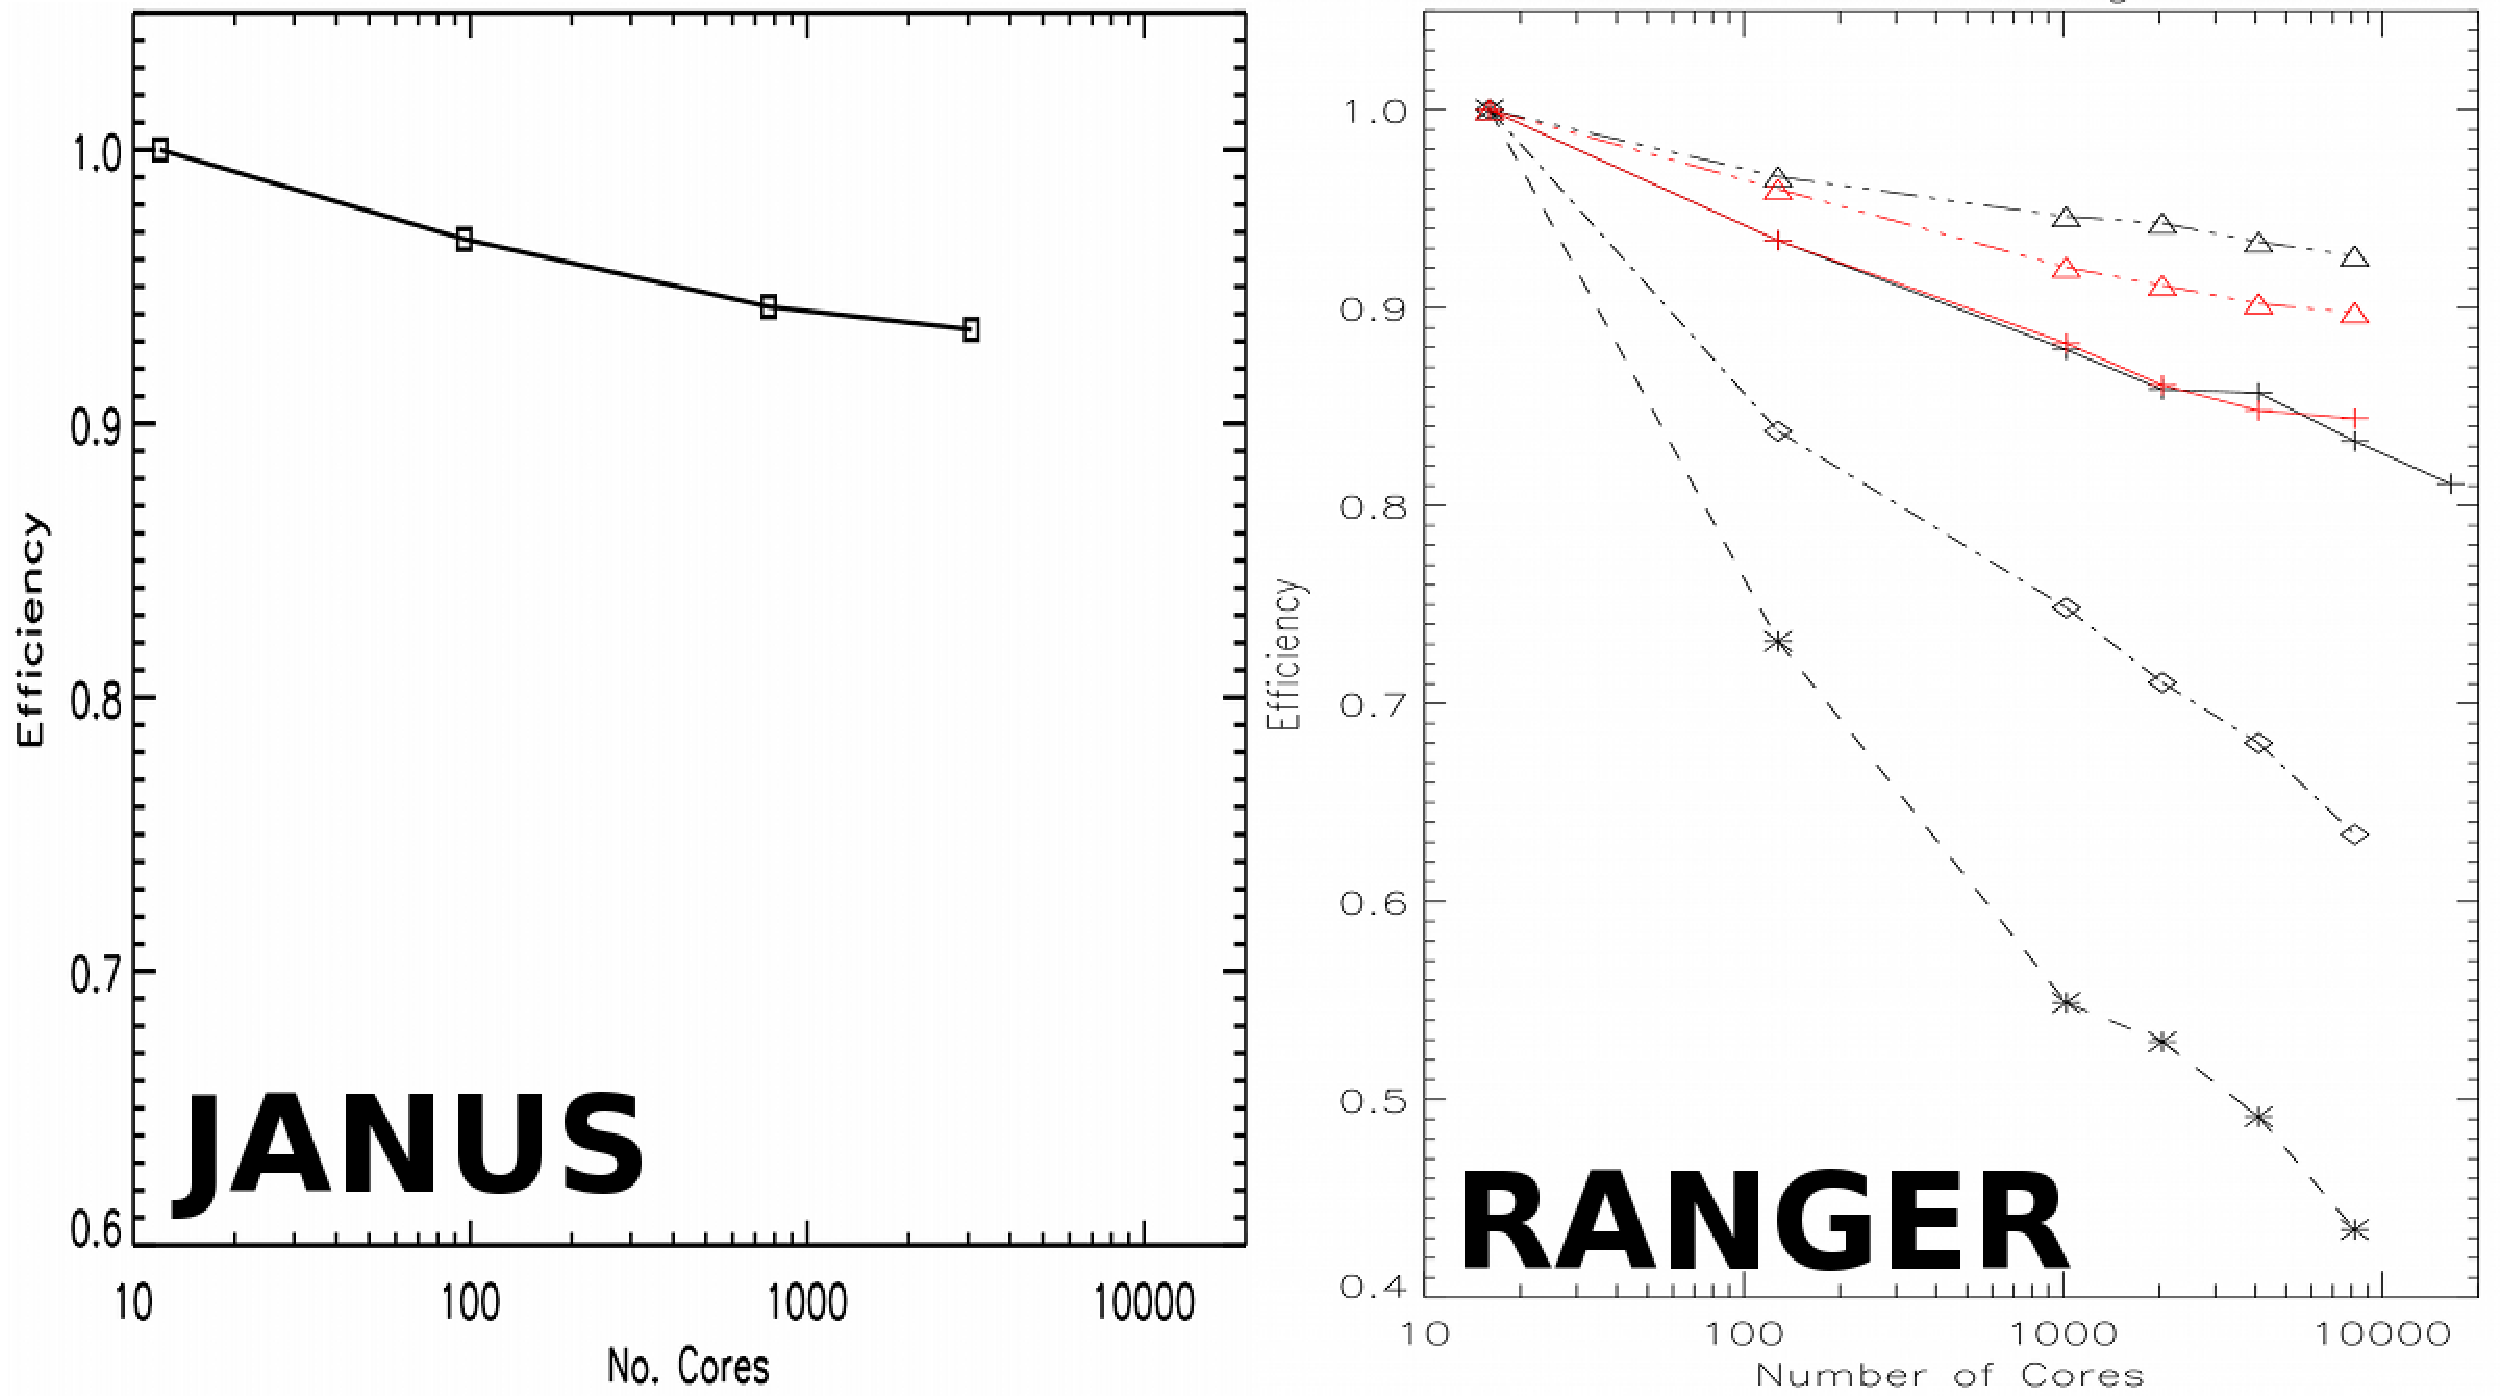
\includegraphics[width=0.5\textwidth]{merged_scaling.pdf}
\vspace{-0.3cm}
\caption{{\footnotesize Weak scaling of {\sc Athena} on {\sc Janus} and {\sc Ranger}.  In the left panel, all points reflect $64^3$ zones per core.  In the right panel, glyphs indicate zones per core: $8^3$ (asterisks), $16^3$ (diamonds), $32^3$ (crosses), or $64^3$ (triangles).  Red lines show a two-level SMR mesh over one half of the domain.}}
\end{center}
\vspace{-0.6cm}
\label{fig:janusscaling}
\end{wrapfigure}

To enable us to estimate the resources our proposed simulations will require, we have constructed performance measures for a high-resolution shearing box simulation run on {\sc Janus} by graduate student Greg Salvesen
in another project that PI Simon is involved in (account UCB00000297). This simulation is designed to extend the work of \cite{simon12} and explore the nature of magnetically dominated accretion disk corona in fully ionized disks. The simulation features essentially identical algorithms (Newtonian MHD in the shearing box limit) to those we propose to use here. They should therefore serve as a reasonable benchmark for the performance of {\sc Athena} on {\sc Janus} for our proposed simulations.


The aforementioned reference simulation was run on a computational grid consisting of $1.7 \times 10^8$ zones utilizing $5184$ cores ($32^3$ zones/core).
Integrating for 24 hours of wall clock time corresponds to $10^5$ cycles.  This leads to a baseline performance of $3.9 \times 10^4$ zone-cycles per CPU second.
From these measures and the quoted {\sc Athena} scaling, we will now estimate the resources required for our proposed runs.


\vspace{-8mm}
\section{Proposed Simulations and Justification of Requested Resources}
\vspace{-2mm}

To explore the nature of turbulence in the dead zone of layered disks, we propose to use {\sc Athena} to run a small set of high-resolution, long-duration shearing box simulations.  The shearing box is a treatment of a local, co-rotating patch of the disk, sufficiently small to be represented by Cartesian coordinates.  The only free parameter in our simulations will be the total surface density.  With a constant active layer surface density, varying the total surface density changes the ratio of active layer to total surface density, which is given by

\begin{equation}
\label{ratio}
\frac{\Sigma_{\rm active}}{\Sigma_{\rm total}} = \frac{1}{2}{\rm ERFC}\left(\frac{z}{H}\right),
\end{equation}

\noindent
where $\Sigma_{\rm active}$ is the active layer surface density, $\Sigma_{\rm total}$ is the total surface density, $H$ is the vertical disk scale height, and ERFC is the complementary error function.  $z$ is the vertical coordinate away from the disk mid-plane where $z = 0$.  By changing the total surface density, we will explore a total of 5 values for this surface density ratio: $\Sigma_{\rm active}/\Sigma_{\rm total} = 1, 10^{-1}, 10^{-2}, 10^{-3}, 10^{-4}$.  A ratio of 1 means that there is no dead zone, and this run will serve as a control study in which the disk will be maximally turbulent for all $z$.  

While $\Sigma_{\rm active}$ remains fixed, the {\it spatial} extent of the active region varies with the ratio of densities as in Equation~(\ref{ratio}).  Using this equation, the surface density ratios (in the above order, but ignoring the first case) correspond to $z/H = 0.91, 1.65, 2.19, 2.63$.   Thus, for all of the MRI modes to be contained within the active layer, the characteristic MRI wavelength must be a fraction of $H$ \citep{hawley95a}.  Furthermore, the characteristic wavelength must be resolved by $\sim 10$ zones \citep{sano04}.  A judicious choice, then, for the characteristic MRI wavelength is $\lambda = 0.25 H = 10 \Delta$, where $\Delta$ is the grid zone size, which we take to be equal in all three dimensions.  These two conditions lead to a resolution requirement of $H/\Delta = 40$; we must have at least 40 zones per $H$ to properly capture and resolve the effects of the MRI in the active layer.  Our proposed simulations will actually have a resolution of $H/\Delta = 48$ since this number is divisible by 12 and thus will fit easily within the {\sc Janus} 12 core architecture (see below). 

\begin{deluxetable}{c c c c c c c}
\label{table}
%\tabletypesize{\small}
\tablecaption{Proposed Simulations}
\tablewidth{\textwidth}
\startdata
\hline \hline
$\Sigma_{\rm active}/\Sigma_{\rm total}$ & \# zones & \# cores & zones/core & Days & {\bf SUs} & {\bf Storage (GB)} \\
\hline
$1$ &  $192\times384\times576$ & 1296 & $32^3$ & 18.3 & ${\bf 0.569\times10^6}$ & {\bf 525} \\
$10^{-1}$ & $192\times384\times576$ & 1296 & $32^3$ & 18.3 & ${\bf 0.569\times10^6}$ & {\bf 525} \\
$10^{-2}$ & $192\times384\times576$ & 1296 & $32^3$ & 18.3 & ${\bf 0.569\times10^6}$ & {\bf 525} \\
$10^{-3}$ & $192\times384\times576$ & 1296 & $32^3$ & 18.3 & ${\bf 0.569\times10^6}$ & {\bf 525} \\
$10^{-4}$ &$ 192\times384\times576$ & 1296 & $32^3$ & 18.3 & ${\bf 0.569\times10^6}$ & {\bf 525} \\
\hline
\vspace{-1mm}
 & & & & {\bf Total} & {$\bf 2.85\times10^6$ {\bf SUs}} & {\bf 2.63 TB} \\
\enddata
\end{deluxetable}

The reference simulation (from account UCB00000297) is being run with a relatively large domain size in order to capture large scale features of the MRI that become dominant in the disk corona \citep{simon12}.  As we are not interested in coronal dynamics here, we will run our simulations at a smaller domain size.  In units of $H$, our domain size will be $4H\times8H\times12H$, which equates to a spatial resolution of $192\times384\times576$.

We will need to run our simulations for many dynamical times (defined by $\Omega^{-1}$, where $\Omega$ is the orbital frequency of the shearing box) in order to achieve statistically significant results.  In particular, we plan to run our simulations for 942 $\Omega^{-1}$ (this equates to 150 orbits).  The average time step in a typical simulation is $5\times10^{-4}\Omega^{-1}$; we will run our simulations for $1.88\times10^6$ time steps. 

As a compromise between an optimal zones per core value and shorter run times, we choose to break our grid up into $32^3$ zones/core so that with a resolution of 48 zones per $H$, we utilize $6 \times 12 \times 18 = 1296$ cores total to span our entire domain.
This number has the advantage of being divisible by 12 so that we can fill 288 {\sc Janus} nodes completely. From this number of cores, the target number of cycles, and the {\sc Janus} performance estimate from the previous section, we can now estimate the resources required for a given high-resolution simulation.

\noindent {\bf The total runtime and cost of a single simulation are:}
\begin{align*}
T_{\rm single} &=\left[\frac{\rm CPU-sec}{3.9 \times 10^4~{\rm zones-cycles}}\right]\frac{(192\times384\times576~{\rm zones}) (1.88 \times 10^6~{\rm cycles})}{1296~{\rm CPU}}\left[\frac{1~{\rm hour}}{3600~{\rm sec}}\right]
           = \mathbf{439}~{\rm \bf hours}, \\
C_{\rm single} &=439~{\rm hours}\times1296~{\rm CPU}=\mathbf{0.569 \times 10^6~{\rm \bf SU}}.
\end{align*}

The proposed runs are summarized in Table 1, with the requested computer time and storage space in bold-face.
We will run all of these simulations in the {\sc Janus} ``wide'' queue in 24-hour batches, taking advantage of {\sc Athena}'s built-in checkpointing system that facilitates restarting after the run is terminated.
Using the storage and memory information from the reference simulation and then dividing by 4 (our grid is 4 times smaller), we calculate a memory and storage requirement for each run of $\sim 0.75$ GB/node and 525 GB, respectively.
Since our total storage requirement is rather large, our strategy will be to stage the data temporarily ($\sim 6$ weeks) on the Lustre scratch system while conducting the analysis. The processed data products (line plots, averages, animations, etc.) will be stored on resources local to our group and/or the {\sc Janus} project spaces. Any essential full data dumps or restart files will be migrated to external long-term storage, such as TACC's {\sc Ranch} system or the NICS HPSS system.

As described above, we intend to conduct five simulations.
We will submit these runs on a regular schedule such that we complete approximately 1-2 simulations per quarter-year, thus avoiding reabsorption of our awarded SUs into the general allocation pool.
The total cost of all proposed models will be $C=5 \times C_{\rm single} =\mathbf{2.85 \times 10^6}$ {\bf SU}.
The total wall clock time required to run all simulations will be $T=5 \times T_{\rm single} =${\bf 2195 hours (or 91 days)}.


\vspace{-8mm}
\section{Computational Resources}
\label{sec:computationalresources}
\vspace{-2mm}
{\sc Janus} is an excellent resource for our proposed simulations because they require regular access to approximately 100 nodes, taking full advantage of {\sc Janus}' fast interconnects.
Locally, our research group has access to 16-core machines that are useful for testing and development, but not for production-level simulations.
We also currently have $\sim 4.4$ million CPU-hours remaining on the NICS {\sc Darter} system through XSEDE (TG-AST120062).  However, this time has been set aside for a completely different project involving the study of accretion at large radii (i.e., beyond the dead zone) in protoplanetary disks.  Furthermore,
{\sc Janus} is a local machine with an excellent help desk system and occasional seminars through the Research Computing division of the University of Colorado.  Since the person responsible for running the proposed 
simulations (co-I Daniel Gold; see below) is relatively new to high performance computing, such excellent local resources will be necessary for Mr. Gold to carry out his tasks.

Analyzing our simulations generally requires only three tools: IDL, VisIt, and yt, all of which we have already used extensively on {\sc Janus}.
The high-memory nodes, in particular, have proven useful in running some of our more memory-intensive post-processing IDL applications to extract and analyze information from the raw simulation data.
While such procedures can be time-consuming, they generally involve only a small number of SUs compared to the total size of the requested allocation.

\vspace{-8mm}
\section{Research Plan}
\vspace{-2mm}
The results of all proposed investigations will be published in refereed journals and presented at scientific conferences, both general and specialized.
Primary responsibility for the setup and execution of the proposed simulations will fall to graduate student Daniel Gold, working under the supervision of PI Dr. Jacob Simon and co-I Prof. Philip Armitage.  Dr. Simon will be responsible for guiding Mr. Gold in running the simulations outlined above and running the proper analyses on the simulation data. Dr. Simon has had extensive experience testing and running similar simulations on {\sc Janus} and has been involved as a PI or Co-I on multiple Teragrid/XSEDE projects (TG-AST120062, TG-AST090106).   Dr. Rebecca Martin will be responsible for interpreting the final results and applying the relationship between disk surface density and dead zone turbulence to semi-analytic, global models of protoplanetary disk evolution.  Dr. Martin is an expert on protoplanetary disks with many publications on global phenomena in these disks, e.g., FU Ori outbursts and large scale instabilities.
Finally, Prof. Armitage will assist with the theoretical interpretation and analysis and will provide supervision to the group as a whole. 


\bibliography{refs}

\end{document}
